\pagestyle{myheadings}

\chapter{Bounds on Quantum Error-Correcting Codes}
\label{chap-bounds}
\markright{CHAPTER~\ref{chap-bounds}. \ BOUNDS ON QUANTUM CODES}

\section{General Bounds}
\label{sec-gen-bounds}
\pagestyle{headings}

The question of how efficient an error-correcting code of a given block size
can be made in terms of both encoded qubits and distance is an interesting
and important question in the theories of both classical and quantum error
correction.  In the classical theory, only upper and lower bounds exist on
the efficiency of codes that must have a given minimum distance between
all codewords.  The true, achievable bounds on such codes are unknown.
Better understood in the classical case is the asymptotic efficiency of coding
(where we only require that the code correct all likely errors).  In the limit
of infinite bits sent, we usually require the code to correct measure one of
the errors occuring using some probability measure associated with the channel.
Classically, Shannon's theorem tells us what the achievable capacity of a
channel is.  No real quantum analogue of Shannon's theorem is known, despite
extensive work on the subject~\cite{lloyd, schumacher, barnum}.

One simple upper bound on the efficiency of quantum codes is the
quantum Hamming bound~\cite{ekert}.  For a nondegenerate code with
basis codewords $\ket{\psi_i}$ and possible errors $E_a$, all of the states
$E_a \ket{\psi_i}$ are linearly independent for all $a$ and $i$.  If the code
uses $n$ qubits, there can only be $2^n$ linearly indepedent vectors in the
Hilbert space, so the number of errors times the number of codewords
must be less than or equal to $2^n$.  If the code corrects all errors of
weight $t$ or less and encodes $k$ qubits, this means
\begin{equation}
	\Sum_{j=0}^{t} 3^j \pmqty{n \\ j} 2^k \leq 2^n.
	\label{eq-QHB-finite}
\end{equation}
There are \mbox{\tiny $\pmqty{n \\ j}$} ways to choose $j$ qubits to be
affected by $j$ errors and $3^j$ ways these errors can be tensor products of
$\X$, $\Y$, and $\Z$.  This bound is completely analogous to the classical
Hamming bound, with two differences: the quantum bound has a factor of $3^j$
reflecting the additional quantum-mechanical degrees of freedom; and the
quantum bound only applies to nondegenerate codes.  The distinction
between degenerate and nondegenerate codes is a purely
quantum-mechanical distinction; there are no classical degenerate codes.
It is unknown whether there are any degenerate codes that exceed the
quantum Hamming bound (\ref{eq-QHB-finite}).

If we let the block size $n$ grow arbitrarily large, we should also increase
the expected number of errors.  Consider the depolarizing channel, which is
equally likely to have $\X$, $\Y$, and $\Z$ errors.  Suppose there is a
probability $p$ of having one of these errors on a given qubit and $1-p$ of
having no error.  The expected number of errors on a block of size $n$ is $t
= np$.  The number of likely errors will be about the number of errors of
length $t$, so the quantum Hamming bound becomes
\begin{equation}
	3^{np} \pmqty{n \\ np} 2^k \leq 2^n.
\end{equation}
Taking the logarithm and rearranging gives us
\begin{equation}
	\frac{k}{n} \leq 1 - p \log_2 3 - H(p).
	\label{eq-QHB}
\end{equation}
Again, $H(x) = - x \log_2 x - (1 - x) \log_2 (1-x)$, as with the asymptotic
form of the classical Hamming bound (\ref{eq-Hamming}).  As with the
classical case, we can achieve the quantum Hamming bound by using
random codes.  Unlike the classical case, this is not always the most
efficient use of the channel, so (\ref{eq-QHB}) does not give the actual
channel capacity of the quantum channel.  I will discuss this question in
greater detail in section~\ref{depolarizing}.

For minimum distance codes, it is not in general possible to achieve the
quantum Hamming bound.  We can set a lower bound, the quantum
Gilbert-Varshamov bound.  Recall that
\begin{equation}
	\bra{\psi_i} E_a^\dagger E_b \ket{\psi_j} = C_{ab} \delta_{ij}
\end{equation}
for a quantum code correcting errors $\{E_a\}$ with basis states
$\ket{\psi_i}$.  The matrix $C_{ab}$ is Hermitian, but is further
constrained by the algebraic relationships of the operators $E_a^\dagger
E_b$.  It is better to consider $C_{ab}$ as a function of operators $O =
E_a^\dagger E_b$.  When the possible errors are all operators of up to
weight $t$, $O$ can be any operator of weight $\leq 2t$.  Slightly more
generally, for a code of distance $d$, $O$ is any operator of weight less
than $d$.  Therefore, the statement
\begin{equation}
	\bra{\psi} E_a^\dagger E_b \ket{\psi} = C_{ab}
	\label{eq-Cab}
\end{equation}
is actually
\begin{equation}
	N = \Sum_{j=0}^{d-1} 3^j \pmqty{n \\ j}
\end{equation}
constraints on the state $\ket{\psi}$.  For generic $C_{ab}$ (satisfying the
appropriate algebraic constraints) and generic linear subspace $V$ with
dimension larger than $N$, there will be states $\ket{\psi}$ satisfying
equation (\ref{eq-Cab}).

Suppose we choose generic $C_{ab}$ and a generic state $\ket{\psi_1}$
satisfying (\ref{eq-Cab}).  Now restrict attention to the subspace
orthogonal to $\ket{\psi_1}$ and to all $O \ket{\psi_1}$ for operators $O$ of
weight less than $d$.  For an $n$-qubit Hilbert space, this subspace has
dimension $2^n - N$.  Choose a generic state $\ket{\psi_2}$ in this subspace
satisfying (\ref{eq-Cab}).  Now restrict attention to the subspace
orthogonal to both $O \ket{\psi_1}$ and $O \ket{\psi_2}$.  We can again
pick $\ket{\psi_3}$ in this subspace satisfying (\ref{eq-Cab}), and so on.
Choose $\ket{\psi_i}$ orthogonal to all $O \ket{\psi_j}$ ($j \leq i-1$) and
satisfying (\ref{eq-Cab}).  We can continue doing this as long as
\begin{equation}
	\Sum_{j=0}^{d-1} 3^j \pmqty{n \\ j} i < 2^n.
\end{equation}
Therefore, we can always find a distance $d$ quantum code encoding $k$
qubits in $n$ qubits satisfying
\begin{equation}
	\Sum_{j=0}^{d-1} 3^j \pmqty{n \\ j} 2^k \geq 2^n.
	\label{eq-QGV}
\end{equation}
This is the quantum Gilbert-Varshamov bound.  In the limit where $t = pn
= d/2$, with $n$ large, this becomes
\begin{equation}
	\frac{k}{n} \geq 1 - 2p \log_2 3 - H(2p).
\end{equation}

The quantum Hamming bound only limits the efficiency of nondegenerate
codes.  For degenerate codes, we can still set a bound, but it will not be as
restrictive.  For an $[n, k, d]$ code, we can choose any $d-1$ qubits and
remove them.  The remaining $n-d+1$ qubits must contain enough
information to reconstruct not only the $2^k$ possible codewords, but the state
of the missing qubits as well.  Because the missing qubits can be any
qubits, we can choose them to have maximum entropy.  Then
\begin{eqnarray}
	n-d+1 & \geq & d-1+k \\
	n & \geq & 2(d-1) + k.
\end{eqnarray}
This is the Knill-Laflamme bound~\cite{knill-laflamme-theory,cerf-cleve}.
It is a quantum analog of the classical Singleton bound.
A code to correct $t$ errors must have distance $d=2t+1$, so for such a
code, $n \geq 4t + k$.  This bound holds for any code with a given
minimum distance, whether it is degenerate or nondegenerate.  For
instance, this bound demonstrates that the smallest one-error-correcting
quantum code uses five qubits.

\section{Weight Enumerators and Linear Programming Bounds}
\label{sec-enumerators}

In the classical theory of error-correcting codes, the distribution of
codeword weights contains a great deal of information about the code.
This distribution is often encoded in the coefficients of a polynomial, and
algebraic relationships between these polynomials, known as {\em weight
enumerators}, can be very useful for setting bounds on classical codes.
Many of the same ideas can be adapted for use with quantum
error-correcting codes~\cite{rains-shadow, shor-laflamme-QMW,
	rains-enumerators, rains-poly-invariants}.

Let $A_d$ be the number of elements of the stabilizer $S$ with weight $d$,
and let $B_d$ be the number of elements of $N(S)$ with weight $d$ (ignoring
overall phases).  Note that $B_d \geq A_d \geq 0$.  Define polynomials
\begin{eqnarray}
	A (z) & = & \Sum_{d=0}^{n} A_d z^d \\
	B (z) & = & \Sum_{d=0}^{n} B_d z^d.
\end{eqnarray}
$A_0 = B_0 = 1$ always.  For a code of distance $d$, $B_{d'} = A_{d'}$ for
all $d' < d$.  For a nondegenerate code, $B_{d'} = A_{d'} = 0$ for $d' < d$.  A
degenerate code has $B_{d'} = A_{d'} > 0$ for at least one $d' < d$.  $A(z)$
and $B(z)$ are the weight enumerators of $S$ and $N(S)$.

The polynomials $A(z)$ and $B(z)$ satisfy the quantum MacWilliams
identity \cite{shor-laflamme-QMW}:
\begin{equation}
	B(z) = \frac{1}{2^{n-k}} (1+3z)^n A \left( \frac{1-z}{1+3z} \right).
	\label{eq-QMW}
\end{equation}
In other words,
\begin{equation}
	\Sum_{d=0}^{n} B_d z^d = \frac{1}{2^{n-k}} \Sum_{d=0}^{n} A_d (1-z)^d
	(1+3z)^{n-d}.
\end{equation}
Matching coefficients of $z^d$, we find
\begin{equation}
	B_d = \frac{1}{2^{n-k}} \Sum_{d'=0}^{n} \left[ \Sum_{s=0}^{d} (-1)^s 3^{d-s}
	\pmqty{d' \\ s} \pmqty{n-d' \\ d-s} \right] A_{d'}.
\end{equation}

To prove this, note that an operator $E \in \G$ of weight $d$ will either
commute with every operator $M \in S$ or it will commute with exactly
half of the operators in $S$.  Therefore, if we sum
\begin{equation}
	\Sum_{M \in S} (-1)^{f_M (E)},
\end{equation}
we will get zero if $E \notin N(S)$ and $2^{n-k}$ if $E \in N(S)$ (recall that
$f_M (E)$ is $0$ if $M$ and $E$ commute and $1$ if they do not).
Therefore, we can write $B_d$ as follows:
\begin{equation}
	B_d = \frac{1}{2^{n-k}} \Sum_{E} \Sum_{M \in S} (-1)^{f_M (E)},
\end{equation}
where the sum over $E$ is taken over all $E \in \G$ of weight $d$.  We
reverse the order of summation and break up the sum over $M$ to the
sum over $d'$ and the sum over $M \in S$ of weight $d'$ to get
\begin{equation}
	B_d = \frac{1}{2^{n-k}} \Sum_{d'=0}^{n} \Sum_M \Sum_E (-1)^{f_M (E)}.
\end{equation}
Now, any given $M$ and $E$ will both act nontrivially on some set of $s$
qubits.  Of those $s$, they will act as different Pauli matrices on $t$ qubits
and as the same Pauli matrix on $s-t$ qubits.  Now,
\begin{equation}
(-1)^{f_M (E)} = (-1)^t.
\end{equation}
The number of operators $E$ that agree with $M$ on $s-t$ qubits and
disagree on $t$ qubits is
\begin{equation}
	1^{s-t} 2^t 3^{d-s} \pmqty{s \\ t} \pmqty{d' \\ s} \pmqty{n-d' \\ d-
	s}.
\end{equation}
Note that this does not depend on $M$.  Thus,
\begin{eqnarray}
	B_d & \!\! = & \!\! \frac{1}{2^{n-k}} \Sum_{d'=0}^{n} \Sum_M \Sum_{s=0}^{d}
	\Sum_{t=0}^{s} \left[1^{s-t} (-2)^t \pmqty{s \\ t}\right] 3^{d-s}
	\pmqty{d' \\ s} \pmqty{n-d' \\ d-s} \\
	& \!\! = & \!\! \frac{1}{2^{n-k}} \Sum_{d'=0}^{n} \Sum_M \Sum_{s=0}^{d} (1 -
	2)^s 3^{d-s} \pmqty{d' \\ s} \pmqty{n-d' \\ d-s} \\
	& \!\! = & \!\! \frac{1}{2^{n-k}} \Sum_{d'=0}^{n} \Sum_M \Sum_{s=0}^{d} (-1)^s
	3^{d-s} \pmqty{d' \\ s} \pmqty{n-d' \\ d-s} \\
	& \!\! = & \!\! \frac{1}{2^{n-k}} \Sum_{d'=0}^{n} \left[ \Sum_{s=0}^{d} (-1)^s
	3^{d-s} \pmqty{d' \\ s} \pmqty{n-d' \\ d-s} \right] A_{d'}.
\end{eqnarray}

This proves the quantum MacWilliams identity (\ref{eq-QMW}) for
stabilizer codes.  The coefficients $A_d$ and $B_d$ can also be defined
for non-stabilizer codes, and equation (\ref{eq-QMW}) will still hold, so
any bounds derived strictly from the quantum MacWilliams identity will
hold for any quantum code, not just stabilizer codes.  For any code of
distance $d$, the coefficients $A_d$ and $B_d$ satisfy the additional
constraints
\begin{eqnarray}
	B_0 & = & A_0 = 1 \\
	B_{d'} & = & A_{d'}\ (d' < d) \\
	B_{d'} & \geq & A_{d'} \geq 0\ (\forall\,d').
\end{eqnarray}
For a nondegenerate code, $A_{d'} = B_{d'} = 0$ for $d' < d$.  These
constraints along with equation (\ref{eq-QMW}) restrict the allowed values
of $A_d$ and $B_d$.  The constraints are all linear, so standard linear
programming techniques will find solutions.  If there are no possible
integer values of $A_d$ and $B_d$ satisfying all of the constraints, there is
no $[n, k, d]$ code.  Otherwise, the possible solutions will give us
parameters of possible codes.  For instance, applying the constraints for a
$[5, 1, 3]$ code produces the unique solution $A_i = (1, 0, 0, 0, 15, 0)$ and
$B_i = (1, 0, 0, 30, 15, 18)$~\cite{shor-laflamme-QMW}.  Therefore, the
usual five-qubit code is essentially the only $[5,1,3]$ code.  There are thus
no degenerate five-qubit codes.

Even tighter linear programming bounds than those produced by the
quantum MacWilliams identity are possible.  This can be done using the
quantum shadow enumerator~\cite{rains-shadow}.  The {\em shadow} $Sh(S)$ of
a code $S$ is defined as the set of $E \in \G$ satisfying
\begin{equation}
	f_M (E) \equiv {\rm wt} (M) \pmod{2}
\end{equation}
for all $M \in S$ (where ${\rm wt} (M)$ is the weight of $M$).  Define
$S_d$ to be the number of elements of $Sh(S)$ of weight $d$ (again, ignoring
overall phases), and
\begin{equation}
	S (z) = \Sum_{d=0}^{n} S_d z^d.
\end{equation}
$S(z)$ is the {\em shadow enumerator} of $S$.  Then
\begin{equation}
	S(z) = \frac{1}{2^{n-k}} (1+3z)^n A \left( \frac{z-1}{1+3z} \right).
	\label{eq-shadow}
\end{equation}

If $S$ contains only operators of even weight, then $E \in Sh(S)$ iff $f_M (E)
= 0$ for all $M \in S$, so $Sh(S) = N(S)$, and $S_d = B_d$.  Furthermore, in
this case, $A(z)$ is an even function, so
\begin{eqnarray}
	S(z) & = & B(z) = \frac{1}{2^{n-k}} (1+3z)^n A \left( \frac{1-z}{1+3z} \right)
	\\
	& = & \frac{1}{2^{n-k}} (1+3z)^n A \left( \frac{z-1}{1+3z} \right).
\end{eqnarray}

If $S$ contains an element of odd weight, consider the subset $S' \subset
S$ of even weight operators.  Then $S'$ has exactly $2^{n-k-1}$ elements.
This is true because in order for $M, M' \in S$ to commute, they must overlap
and disagree only on an even number of qubits.  Thus, ${\rm wt}(MM') \equiv
{\rm wt}(M) + {\rm wt}(M') \pmod{2}$.
The shadow of $S$ is just $Sh(S) = N(S') - N(S)$.  Let $B'(z)$ and $A'(z)$ be
the weight enumerators of $S'$ and $N(S')$.  Then
\begin{eqnarray}
	S(z) & = & B' (z) - B(z) \\
	& = & \frac{1}{2^{n-k-1}} (1+3z)^n A' \left( \frac{1-z}{1+3z} \right) -
	\frac{1}{2^{n-k}} (1+3z)^n A \left( \frac{1-z}{1+3z} \right) \nonumber \\ \\
	& = & \frac{1}{2^{n-k}} (1+3z)^n \left[ 2 A' \left( \frac{1-z}{1+3z} \right) -
	A \left( \frac{1-z}{1+3z} \right) \right].
\end{eqnarray}
Now, $A'_d = A_d$ for even $d$ and $A'_d = 0$ for odd $d$, so $A(z) + A(-
z) = 2 A'(z)$, and
\begin{equation}
	S(z) = \frac{1}{2^{n-k}} (1+3z)^n A \left( \frac{z-1}{1+3z} \right).
\end{equation}

Again, the shadow enumerator can be defined for non-stabilizer codes and
satisfies the same relationship with $A(z)$ as for stabilizer codes.  In both
the stabilizer and non-stabilizer case, $S_d \geq 0$.  Along with
(\ref{eq-shadow}), this provides additional constraints for the linear
programming bound restricting the parameters of any code.  These bounds
have been applied to all possible codes with $n \leq 30$
\cite{rains-shadow,calderbank-GF4}.  Among other things, they show that
the smallest possible distance five code is an $[11,1,5]$ code and that
degenerate codes in this region all fall below the quantum Hamming
bound.  The shadow enumerator can also be used to show that any nondegenerate
code on $n$ qubits can correct at most $\lfloor \frac{n+1}{6} \rfloor$
errors~\cite{rains-shadow}.

\section{Bounds on Degenerate Stabilizer Codes}

It is still unknown whether there are any degenerate codes that exceed the
limits set by the quantum Hamming bound, but for certain restricted cases,
we can show that there are not.  For codes using fewer than 30 qubits, the
linear programming bounds of the previous section show this.  In this
section, I will show that the statement also is true for all stabilizer codes
that correct one or two errors.  The results can be extended slightly
beyond stabilizer codes, but do not apply to the most general possible code.

For a one-error-correcting degenerate code, the stabilizer $S$ will contain
one or more operators of weight one or two.  Weight one operators totally
constrain a qubit and both the operator and the qubit can be eliminated,
converting an $[n, k, d]$ code into an $[n-1, k, d]$.  If the latter satisfies
the quantum Hamming bound, the former will as well.  Suppose there are $l$
independent weight two operators $M_1, \ldots, M_l$ in $S$.  Let $D$ be the
group generated by $M_1, \ldots, M_l$.  Note that $S - D$ will contain no
operators of weight less than three.  The weight two operators in $D$ tell us
which errors produce the same states.  For instance, if $M_1 = \Zs{1} \Zs{2}$,
$\Zs{1} \ket{\psi} = \Zs{2} \ket{\psi}$ for any codeword $\ket{\psi}$.

Any operator in $N(D)$ will take states fixed by $D$ to states fixed by $D$.
The total dimensionality of the subspace fixed by $D$ is $2^{n-l}$.  Suppose
that none of the operators in $D$ acts on some qubit $j$.  Then all of the
three operators $\Xs{j}$, $\Ys{j}$, and $\Zs{j}$ are in $N(D)$, and they are
not degenerate.  Therefore, they must produce orthogonal states in the
subspace fixed by $D$ for each basis codeword.  There are always at least
$n-2l$ qubits not affected by $D$, since each generator of $D$ can add at
most two qubits.  Therefore,
\begin{eqnarray}
	\left[1 + 3(n-2l) \right] 2^k & \leq & 2^{n-l} \\
	k & \leq & n - l - \log_2 [1+3(n-2l)]. \label{eq-QHB-deg1}
\end{eqnarray}
Recall that the quantum Hamming bound says that
\begin{equation}
	k \leq n - \log_2 (1+3n),
\end{equation}
so (\ref{eq-QHB-deg1}) is more restrictive when
\begin{eqnarray}
	l + \log_2 [1+3(n-2l)] & \geq & \log_2 (1+3n) \\
	l & \geq & \log_2 \left[ \frac{1+3n}{1+3(n-2l)} \right] \\
	& = & \log_2 \left[ 1 + \frac{6l}{1 + 3(n-2l)} \right]. \label{eq-QHB-deg1'}
\end{eqnarray}
Assuming $n \geq 2l$, we see that the quantum Hamming bound will still
hold if $l \geq \log_2 (1+6l)$.  This is true for $l \geq 5$.  For $l=4$,
(\ref{eq-QHB-deg1'}) holds for $n \geq 9$; for $l=3$, it holds for $n \geq
7$.  For $l=2$, (\ref{eq-QHB-deg1'}) holds for $n \geq 5$, and for $l=1$, it
holds for $n \geq 4$.  The remaining possibilities with $n \geq 2l$ are
ruled out by the linear programming bounds of section
\ref{sec-enumerators}.  On the other hand, if $l > n/2$, then $k \leq n-l
\leq n/2$.  For $n \geq 13$, the quantum Hamming bound is less
restrictive than this, so in conjunction with the linear programming
bounds, we can conclude that there are no distance three degenerate stabilizer
codes that exceed the quantum Hamming bound.

We can make a similar argument for codes to correct two errors.  Now let $D$
be generated by the operators of weight four or less in $S$.  There must be
at least $n-4l$ qubits that are unaffected by operators in $D$.  All the
possible weight one and two errors on those qubits give orthogonal states, so
\begin{eqnarray}
	\left[1 + 3(n-4l) + \frac{9}{2} (n-4l) (n-4l-1)\right] 2^k & \leq & 2^{n-l} \\
	\left[1 - \frac{3}{2} n + \frac{9}{2} n^2 + 6 l (1 + 12 l - 6 n)\right] 2^l & \leq & 2^{n-k}.
\end{eqnarray}
The quantum Hamming bound will still hold if
\begin{eqnarray}
	\left[1 - \frac{3}{2}n + \frac{9}{2} n^2 + 6 l (1 + 12 l - 6 n)\right] 2^l &
	\geq & 1 - \frac{3}{2}n + \frac{9}{2} n^2 \\
	\left[ 1 - \frac{6l (6n - 12 l - 1)}{1 - 3n/2 + 9n^2/2} \right] 2^l & \geq & 1.
	\label{eq-QHB-deg2}
\end{eqnarray}
Now, $l (6n - 12 l - 1) = -12 [l^2 - (6n-1) l /12]$ is maximized for $l = (6n-
1)/24$.  That means (\ref{eq-QHB-deg2}) will be satisfied when
\begin{eqnarray}
	\left[ 1 - \frac{(6n - 1)^2}{8 - 12n + 36n^2} \right] 2^l & \geq & 1 \\
	\frac{7}{8 - 12n + 36n^2}\,2^l & \geq & 1 \\
	7 \cdot 2^{l-2} & \geq & 9n^2 - 3n + 2.
\end{eqnarray}
If this is true, the code will satisfy the quantum Hamming bound.  If it is
	{\em not} true, then
\begin{eqnarray}
	l & \leq & 2 - \log_2 7 + \log_2 (9n^2 - 3n + 2) \\
	& \leq & 3 + 2 \log_2 n.
\end{eqnarray}
Then $l (6n - 12l - 1) \leq 6 n l \leq 6 n (3 + 2 \log_2 n)$, so equation
(\ref{eq-QHB-deg2}) will again be satisfied when
\begin{equation}
	\left[ 1 - \frac{6 n (3 + 2 \log_2 n)}{1 - 3n/2 + 9n^2/2} \right] 2^l \geq 1.
\end{equation}
However, for $n \geq 30$,
\begin{equation}
	\frac{6 n (3 + 2 \log_2 n)}{1 - 3n/2 + 9n^2/2} \leq 0.58,
\end{equation}
so (\ref{eq-QHB-deg2}) will be satisfied for any $l$ with $1 < l \leq n/4$
in the regime of interest.  When $l=1$, (\ref{eq-QHB-deg2}) becomes
\begin{equation}
	1 - \frac{6 (6n - 13)}{1 - 3n/2 + 9n^2/2} \geq 1/2.
\end{equation}
However, for $n \geq 30$,
\begin{equation}
	\frac{6 (6n - 13)}{1 - 3n/2 + 9n^2/2} \leq 0.26,
\end{equation}
so (\ref{eq-QHB-deg2}) is satisfied for $l=1$ as well.

Therefore, we are left with $l > n/4$.  Again, this implies that $k \leq n-l <
3n/4$.  This is at least as restrictive than the quantum Hamming bound for $n
\geq 52$.  For $n=31$, the quantum Hamming bound says $k \leq n-13$.
Therefore, for $31 \leq n \leq 51$, the only remaining region of interest,
the code must have $l \leq n/4 + 5$ to violate the quantum Hamming bound.
The only possibility for $l > n/4 + 4$ is $l=12$, $n=31$.  Assume for the
moment that $l \leq n/4 + 4$.  Then there are at least $n - 16$ qubits in
the code that are affected by at most one of the generators of $D$.  This is
more than $l+3$, so either at least two of the generators of $D$ must each
affect two qubits that are fixed by all of the other generators, or one generator fixes four qubits that are unaffected by all of the other generators.
The second case will be more restrictive to the code than the first one, so I
will assume the first case holds.  Assume without loss of generality that the
two generators are $M_{l-1}$ and $M_l$.  Then errors on the four qubits
affected only by these generators leave the codewords within the subspace fixed
by $D'$, the group generated by $M_1, \ldots, M_{l-2}$.  There are 67 errors of
weight zero, one and two on the four qubits, so
\begin{eqnarray}
	67 \cdot 2^k & \leq & 2^{n-(l-2)} \\
	k & \leq & n - l - 5.
\end{eqnarray}
This is at least as restrictive as the quantum Hamming bound for any $n$
between 31 and 51.

That leaves the case $l=12$, $n=31$.  Even in this case, there must be at
least fourteen qubits that are affected by at most one of the generators of
$D$.  As before, this is enough to ensure that we can pick two generators of
$D$ that will together act on four qubits unaffected by any of the other
generators.  Again, $k \leq n - l - 5$, which is more restrictive than the quantum Hamming bound.  Therefore, there are no two-error-correcting degenerate
stabilizer codes exceeding the quantum Hamming bound.

The methods of this section could be adapted and perhaps applied to codes
correcting three or more errors, but it gets more difficult for each
additional error, since the cases with $l > n/(2t)$ must be treated on a
special basis, and the range of $n$ for which this could violate the
quantum Hamming bound grows rapidly with $t$.  Eventually, it might
well be true that some code with enough degeneracies does violate the
quantum Hamming bound.

Even though we cannot rule out the possibility of a sufficiently large
degenerate code violating the quantum Hamming bound, we can still set
a less restrictive bound on degenerate stabilizer codes by constructing
a classical code from the quantum code~\cite{cleve-classical}.  Since bounds
on the efficiencies of classical codes are known, we can therefore get
bounds on the possible parameters of quantum codes.

To produce a classical code from a quantum code, first put the code in
standard form, as per (\ref{eq-standard-form}).  In particular, note the
$r \times k$ matrix $A_2$.  $r \leq n-k$, but by performing single qubit
rotations from $N(\G)$, we can always convert one generator to the product of
$\Z$'s, so we can ensure that $r \leq n-k-1$.  If we look at the classical code
$C$ with $k \times (r+k)$ generator matrix $(A_2^T | I)$, then $C$ encodes
$k$ bits in at most $n-1$ bits.  If the original quantum code could correct
$t$ quantum errors, it turns out that the classical code $C$ can correct $t$
classical bit flip errors, whether the quantum code was degenerate or
nondegenerate.  Therefore, the existence of an $[n, k, d]$ quantum code
implies that an $[n-1, k, d]$ classical code exists.

\section{Error-Correcting Codes and Entanglement Purification Protocols}

Before discussing bounds on the channel capacity, I will discuss another
way of looking at quantum codes that is sometimes helpful for thinking
about the channel capacity.  Consider the situation where Alice prepares a
number of EPR pairs and sends one member of the pair to Bob.  In general,
both the qubits that Alice keeps and the qubits she sends to Bob may be
subject to errors and decoherence.  This means that Alice and Bob will
share a number of imperfect pairs.  If Alice attempts to teleport a state
using these imperfect EPR pairs, for instance, the state that Bob receives
will be incorrect.  Alice and Bob wish to perform some local operations on
their halves of the imperfect pairs so that they are left with a smaller
number of perfect pairs (or at least better ones).  A protocol to do this is
called an {\em entanglement purification protocol} (or EPP)
\cite{bennett-tome,bennett-EPP}.

Depending on the situation, Bob and Alice may or may not be allowed to
communicate with each other and perform operations conditioned on the
results of measurements by the other one.  If both Bob and Alice can
communicate with each other via classical communication channels, the
possible protocols they can implement are called two-way error purification
protocols (or 2-EPPs).  If Bob can only receive classical information (as well
as qubits) from Alice, but not transmit, then Bob and Alice are restricted to
using one-way error purification protocols (or 1-EPPs).  In principle, there is
another possibility.  Bob and Alice might not be able to communicate
classically at all.  However, it turns out that the protocols available for
them in this case are equivalent to the 1-EPPs.  On the other hand, it is
known that in some circumstances, 2-EPPs allow more good pairs to be
purified than 1-EPPs do~\cite{bennett-tome}.

One remarkable fact about 1-EPPs is that they are equivalent to
quantum error-correcting codes.  Suppose we have a quantum code.  We
can make a 1-EPP out of it as follows: Alice encodes the qubits she is going
to send to Bob using the code, then Bob corrects and decodes.  The encoded
qubits that are thus preserved in the channel retain their entanglement
with the qubits Alice kept, and thus form part of a good EPR pair.  The
number of good pairs is just equal to the number of encoded qubits.

Conversely, suppose we have a 1-EPP that distills $k$ good pairs from $n$
noisy pairs and we wish to make a quantum code.  In this case Alice is the
encoder and Bob is the decoder for the code.  Alice creates $n$ EPR pairs
and sends them to Bob, then performs her half of the 1-EPP.  Since she
cannot receive transmissions from Bob, she does not need to wait until Bob
receives the qubits to do this.  This is why a quantum code is equivalent to
a 1-EPP and not a 2-EPP.  After she has performed her half of the
purification protocol, sending any necessary classical information, she
takes the $k$ qubits she wishes to protect and performs her half of the
teleportation protocol using her half of what will be the $k$ good pairs.
Again, she sends the classical information about the measurement results
to Bob.  Bob now receives the qubits, plus all the classical information.  He
completes the purification protocol, purifying $k$ good pairs.  Since they
are good EPR pairs, when he then completes the teleportation protocol, the
resulting state is the correct one, and the whole process acts like a code
encoding $k$ qubits in $n$ qubits.

\section{Capacity of the Erasure Channel}

Most quantum channels are very difficult to analyze.  However, the
channel capacity is known for at least one simple channel of interest.  The
	{\em erasure channel} is the channel for which every qubit sent through the
channel has some chance $p$ of being totally randomized.  However, when
this happens, we always know on which qubit it occurred.  The capacity of
the erasure channel for both quantum codes and 2-EPPs is straightforward
to calculate~\cite{bennett-erasure}.

The capacity for 2-EPPs is particularly straightforward.  If Alice sends $n$
EPR pairs through the channel, $pn$ of them will be destroyed, but $(1-
p)n$ will remain intact.  Furthermore, Bob will know which pairs remain
intact, so he tells Alice and they discard the useless pairs.  This achieves a
rate of $1-p$.  Clearly, it is impossible to do better than this.  This means
that the capacity for a 2-EPP is just $1-p$.

With a 1-EPP or quantum code, we cannot do as well, because Bob cannot
tell Alice which pairs she should keep and which she should throw away.  In
fact, we can set an upper bound on the capacity of $1-2p$.  Suppose the erasure
rate of $p$ in the channel is actually caused by Charlie, who steals any
given qubit with probability $p$, replaces any stolen qubits with random
ones, and then tells Bob which qubits he stole.  When $p = 1/2$, Bob has
exactly the same number of valid pairs as Charlie.  If there were any
operations Alice could make without consulting Bob that enabled him to
purify even a single valid pair, Charlie could do the same thing as Bob, also
giving a valid pair.  Now when Alice attempts to teleport something to Bob,
she is also teleporting it to Charlie.  This would allow the cloning of a
quantum state.  Therefore, the rate for $p>1/2$ is zero.  For $p<1/2$, we
can imagine Alice somehow knows $n(1-2p)$ of the pairs that will not be
stolen by Charlie.  The remaining $2pn$ pairs she is uncertain about.  Of
them, $pn$ will be stolen by Charlie, again leaving him with the same
number of good pairs from this set as Bob has.  If Alice attempts to purify
more than $n(1-2p)$ pairs with Bob, she will therefore also be purifying
pairs with Charlie, again leading to state cloning.  Therefore, the capacity is
bounded above by $1-2p$.

This is, in fact, the actual achievable capacity for this channel.  Suppose we
take a random Abelian subgroup of $\G_n$ with $n-k$ generators.  This
subgroup will act as the stabilizer $S$ of a code.  If we encode $k$ qubits
using this code, and then send them through the erasure channel, for large
$n$, with high probability, $pn$ known qubits will have been randomized.
We need to distinguish between the $4^{pn}$ possible errors on these
qubits.  Since the error operators are all on the same $pn$ qubits, there are
again $4^{pn}$ products of these operators.  If measure one of these products
anticommute with some element of $S$, then we will be able to correct the
errors and decode the $k$ qubits, with fidelity approaching one for large $n$.
Since the generators are chosen randomly, each one will commute with half of
the possible operators of weight $pn$ and anticommute with half of the possible
operators.  The different generators commute and anticommute with operators
independently, so the number of operators that commute with all $n-k$
generators is
\begin{equation}
	4^{pn} / 2^{n-k} = 2^{k - (1-2p)n} = 2^{(r - 1 + 2p) n},
\end{equation}
where $r$ is the rate: $k = rn$.  As long as $r < 1 - 2p$, the chance of not
being able to distinguish all the likely errors goes to zero as $n \rightarrow
\infty$.  Therefore, a random stabilizer code can give us rate $1-2p$.  Since
this coincides with the upper bound on the capacity, it is the actual
capacity of the erasure channel.

\section{Capacity of the Depolarizing Channel}
\label{depolarizing}

The {\em depolarizing channel} is a very natural channel to consider.  In this
channel, with probability $1-p$, each qubit is left alone.  In addition, there
are equal probabilities $p/3$ that $\X$, $\Y$, or $\Z$ affects the qubit.  We
can apply similar methods to the depolarizing channel as with the erasure
channel to place upper and lower bounds on its capacity.  However,
currently these bounds do not meet, so the actual capacity of the
depolarizing channel is unknown.

The depolarizing channel can also simulated by imagining Charlie is
randomly stealing some qubits from the channel.  If Charlie steals a qubit
with probability $q$ and replaces it with a random qubit (not telling Bob
which one was stolen), there is still a $1/4$ chance that Charlie happens to
replace the stolen qubit with one in the same state.  There is only a chance
$q/4$ of Charlie applying each of $\X$, $\Y$, and $\Z$.  Therefore, this
situation corresponds to the depolarizing channel with $p = 3q/4$.  We can
make a cloning argument just as with the erasure channel to set an upper
bound on the capacity.  Again we find that the capacity is limited by $1-2q
= 1- 8p/3$.  When $p > 3/8$, the rate of transmission is necessarily zero.

Actually, we can set a tighter upper bound than this.  Randomly stealing qubits
is not the best eavesdropping method available to Charlie that will look like
the depolarizing channel.  The best eavesdropping method actually allows
him to produce the same state as Bob whenever $p > 1/4$~\cite{fuchs-KL}.
This means that the rate is limited to $1-4p$.  This is the asymptotic form
of the Knill-Laflamme bound, which was derived for codes with a fixed
minimum distance in section~\ref{sec-gen-bounds}.

We can set a lower bound for the achievable rate by again considering the
rate for a random stabilizer code.  If we encode $k$ qubits in $n$ qubits
using a random stabilizer $S$, the expected number of errors is $pn$.  We
need measure one of the errors to be distinguishable from each other.  The
errors $E$ and $F$ are distinguishable if $E^\dagger F$ anticommutes with
some elements of $S$, and are not if they do not.  The typical product
$E^\dagger F$ actually does not have weight $2pn$.  There is a chance
$p^2$ that $E$ and $F$ will both have nontrivial action on a given
qubit.  If they act as different Pauli matrices, the product will still act on
that qubit.  If they act as the same Pauli matrix, the product will not act on
that qubit at all.  The probability of having both act as the same Pauli
matrix is $p^2/3$.  Therefore, the expected length of the product
$E^\dagger F$ is $(2p - 4p^2/3)n$.  Let $x = 2p - 4p^2/3$.

Let the number of errors of weight $w$ be $N(w)$.  Then the number of
different products of weight $xn$ is $N(xn)$, and therefore the number of
typical products that commute with everything in $S$ is $N(xn) / 2^{n-k}$.
Now, there are $N(pn)$ likely errors, so the number of ways we can pair
them into products is $N(pn) [N(pn) -1]/2$.  This means that the number of
ways of getting any given operator $O$ of weight $xn$ is
\begin{equation}
	\left. \pmqty{ N(pn) \\ 2} \right/ N(xn).
\end{equation}
For each of the pairs that gives one of the $N(xn)/2^{n-k}$ products that
commute with $S$, we must remove one of the errors in the pair from the
group of likely errors.  Therefore, we must remove
\begin{equation}
	\left. \pmqty{ N(pn) \\ 2} \right/ 2^{n-k}
\end{equation}
errors.  We want to remove only measure zero of the errors, so we wish this
number to be small compared to $N(pn)$ for large $n$.  Thus,
\begin{eqnarray}
	N (pn) / 2^{n-k+1} & \ll & 1 \\
	N (pn) & \ll & 2^{n-k+1} \\
	k/n & < & 1 - \frac{1}{n} \log_2 N (pn) = 1 - p \log_2 3 - H(p).
\end{eqnarray}
This is just the quantum Hamming bound (\ref{eq-QHB}).  In other words,
a random code saturates the quantum Hamming bound.

However, the quantum Hamming bound only limits the efficiency of
nondegenerate codes.  The typical element of a random stabilizer will have
weight $3n/4$, which is much larger than $pn$ for any $p$ where the rate
could possibly be nonzero.  Therefore, a random code will have a
negligable number of degenerate errors, and the quantum Hamming bound
will still apply.  However, if we choose the stabilizer to be of a restricted
form rather than totally random, we can choose it to have very many
degeneracies, and the quantum Hamming bound may be exceeded
\cite{shor-smolin}, although existing codes only allow us to exceed the
rate of a random code by a very small amount.  Shor and Smolin showed that
by concatenating a random code with a simple repetition code ($\ket{0}$
becomes the tensor product of $\ket{0}$'s and $\ket{1}$ becomes the tensor
product of $\ket{1}$'s), the rate of the code is improved slightly near the
zero-rate limit.  The optimum block size for repetition turns out to be five.

We can still set an upper bound on the efficiency of a degenerate stabilizer
code using similar arguments to those that gave us the capacity of a
random stabilizer code.  Note that this upper bound does not necessarily
apply to all codes, so it may not be a strict upper bound on the capacity.
However, non-stabilizer codes are very difficult to work with, so it does
provide a practical upper bound on the capacity.

To give this bound, assume that every element of $S$ actually has weight
$xn$.  This bound is unlikely to be achievable, since the product of two
operators of weight $xn$ will only rarely have weight $xn$ again.  There
are at least $N(xn)/2^{n-k}$ operators of weight $n$ that commute with $S$,
but $2^{n-k}$ of them are in $S$.  Therefore, in the best case, there are only
$N(xn)/2^{n-k} - 2^{n-k}$ operators that can potentially cause a problem.  In
the limit where $n$ and $k = rn$ are both large, either $N(xn)/2^{n-k}$ will
dominate the number of troublesome operators, or $N(xn)/2^{n-k} \ll 2^{n-
k}$.  In the first case, the calculation goes through as for a completely
random stabilizer, giving us a capacity only at the quantum Hamming
bound.  In the second case,
\begin{eqnarray}
	N(xn) & \ll & 2^{2(n-k)} \\
	r = k/n & < & 1 - \frac{1}{2n} \log_2 N(xn) = 1 - \frac{x}{2} \log_2 3 -
	\frac{1}{2} H(x).
	\label{eq-deg-bound}
\end{eqnarray}
Since $x = 2p - 4p^2/3$, this is higher than the quantum Hamming bound.
Equation (\ref{eq-deg-bound}) gives an upper bound on the capacity of the
depolarizing channel achievable using stabilizer codes.  It is shown in
figure~\ref{CCBounds} along with the Knill-Laflamme bound and the quantum
Hamming bound.  Cleve has also proved a bound on the capacity achievable
using degenerate stabilizer codes \cite{cleve-classical}, but it is slightly
worse than (\ref{eq-deg-bound}) everywhere in the region of interest, so
it is not shown in the figure.
\begin{figure}
	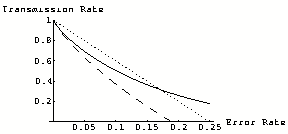
\includegraphics{Capacity.png}
	\caption[The quantum Hamming bound, the Knill-Laflamme bound, and the bound
	from equation~(\ref{eq-deg-bound})]{The quantum Hamming bound (dashed), the
	Knill-Laflamme bound (dotted), and the bound from equation~(\ref{eq-deg-bound})
		(solid).}
	\label{CCBounds}
\end{figure}